\clearpage
\chapter*{Evidencia GA1-220501092-AA5-EV02: Informe de Validación (Prototipos y Casos de Prueba)}
\phantomsection
\addcontentsline{toc}{chapter}{Evidencia GA1-220501092-AA5-EV02: Informe de Validación (Prototipos y Casos de Prueba)}
\setcounter{section}{0}

\section{Introducción}

El presente informe detalla el proceso de \textbf{Evaluación y Validación} de cuatro Historias de Usuario (HU) seleccionadas como críticas para el proyecto de modernización del sistema de gestión de mantenimiento y activos. Este proceso incluyó la creación de \textbf{prototipos de baja fidelidad (\textit{mockups})} en Figma, que sirven como herramienta visual para validar la comprensión de los requisitos funcionales y establecer la base para los \textbf{Casos de Prueba}.

\section{Abreviaturas y Glosario Técnico}

\begin{center}
\begin{tabular}{|l|p{10cm}|}
\hline
\textbf{Abreviatura} & \textbf{Significado} \\ \hline
\textbf{HU} & Historia de Usuario \\ \hline
\textbf{KPI} & Key Performance Indicator (Indicador Clave de Desempeño) \\ \hline
\textbf{MTBF} & Mean Time Between Failures (Tiempo Medio Entre Fallos) \\ \hline
\textbf{MTTR} & Mean Time To Repair (Tiempo Medio de Reparación) \\ \hline
\textbf{MTTO} & Mantenimiento \\ \hline
\textbf{CP} & Caso de Prueba \\ \hline
\textbf{3D} & Tres Dimensiones \\ \hline
\end{tabular}
\end{center}

\section{Alcance del Documento}

El alcance de este informe se limita a la validación de los siguientes cuatro requerimientos, abarcando diferentes roles y funcionalidades clave del sistema:

\begin{center}
\footnotesize
\begin{tabular}{|l|l|p{5cm}|p{3.5cm}|}
\hline
\textbf{ID HU} & \textbf{Rol} & \textbf{Descripción del Requerimiento} & \textbf{Tipo de Prototipo} \\ \hline
\textbf{MTTO-001} & Planificador & Programación de Mantenimiento Preventivo (mensual o trimestral) & Formulario (Escritorio) \\ \hline
\textbf{ADM-017} & Gerente & Dashboard ejecutivo de KPIs (MTBF, MTTR, Costos) & Dashboard (Escritorio) \\ \hline
\textbf{INV-021} & Jefe de Almacén & Alertas de Stock Crítico (poder configurar el mínimo) & Panel de Configuración (Escritorio) \\ \hline
\textbf{VIS-010} & Técnico & Visualización de Despiece de Activo & \textbf{Visor de Activos (Móvil/Tablet)} \\ \hline
\end{tabular}
\end{center}
\normalsize

\section{Prototipos de Baja Fidelidad (Evidencia Visual)}

A continuación, se presentan las cuatro visualizaciones creadas para la validación de los requerimientos.

\subsection{P-MTTO-001: Programación de Mantenimiento}

\begin{figure}[H]
    \centering
    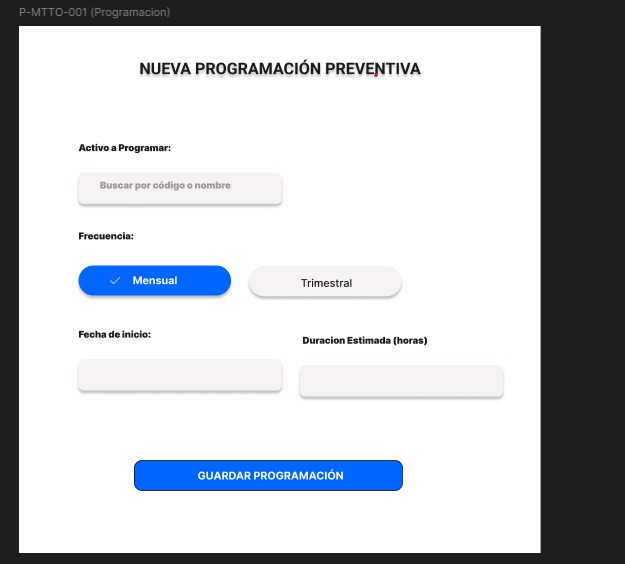
\includegraphics[width=0.9\textwidth]{assets/proto_mtto_prog.jpeg}
    \caption{Prototipo P-MTTO-001}
\end{figure}

\begin{itemize}
    \item \textbf{Validación:} El diseño incluye la selección de \textbf{Frecuencia (Mensual/Trimestral)} y los campos de entrada requeridos, validando la funcionalidad clave.
\end{itemize}

\subsection{P-ADM-017: Dashboard Ejecutivo de KPIs}

\begin{figure}[H]
    \centering
    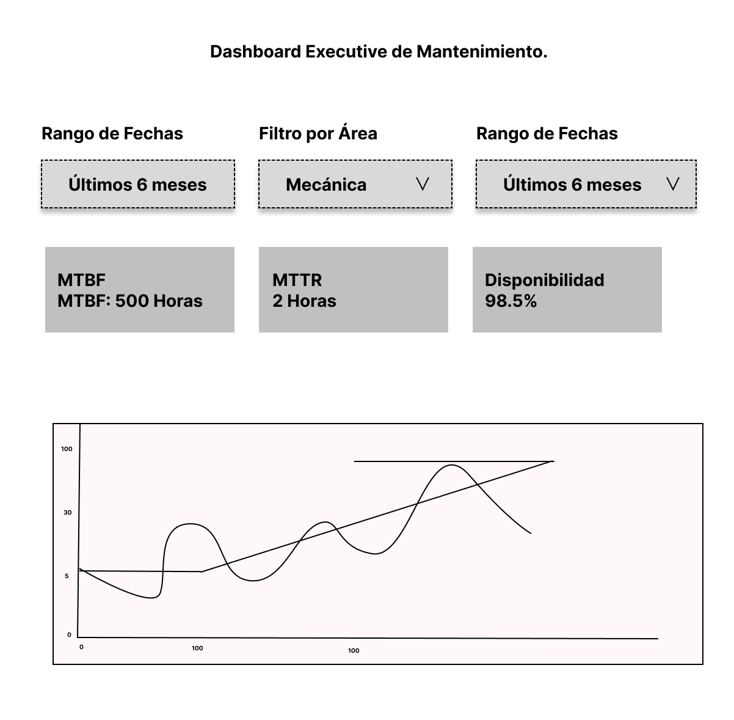
\includegraphics[width=0.9\textwidth]{assets/proto_dashboard.png}
    \caption{Prototipo P-ADM-017}
\end{figure}

\begin{itemize}
    \item \textbf{Validación:} El Dashboard presenta los \textbf{KPIs (MTBF, MTTR)} y los elementos de filtro de fecha y área, cumpliendo con la necesidad gerencial de análisis.
\end{itemize}

\subsection{P-INV-021: Alertas de Stock Crítico}

\begin{figure}[H]
    \centering
    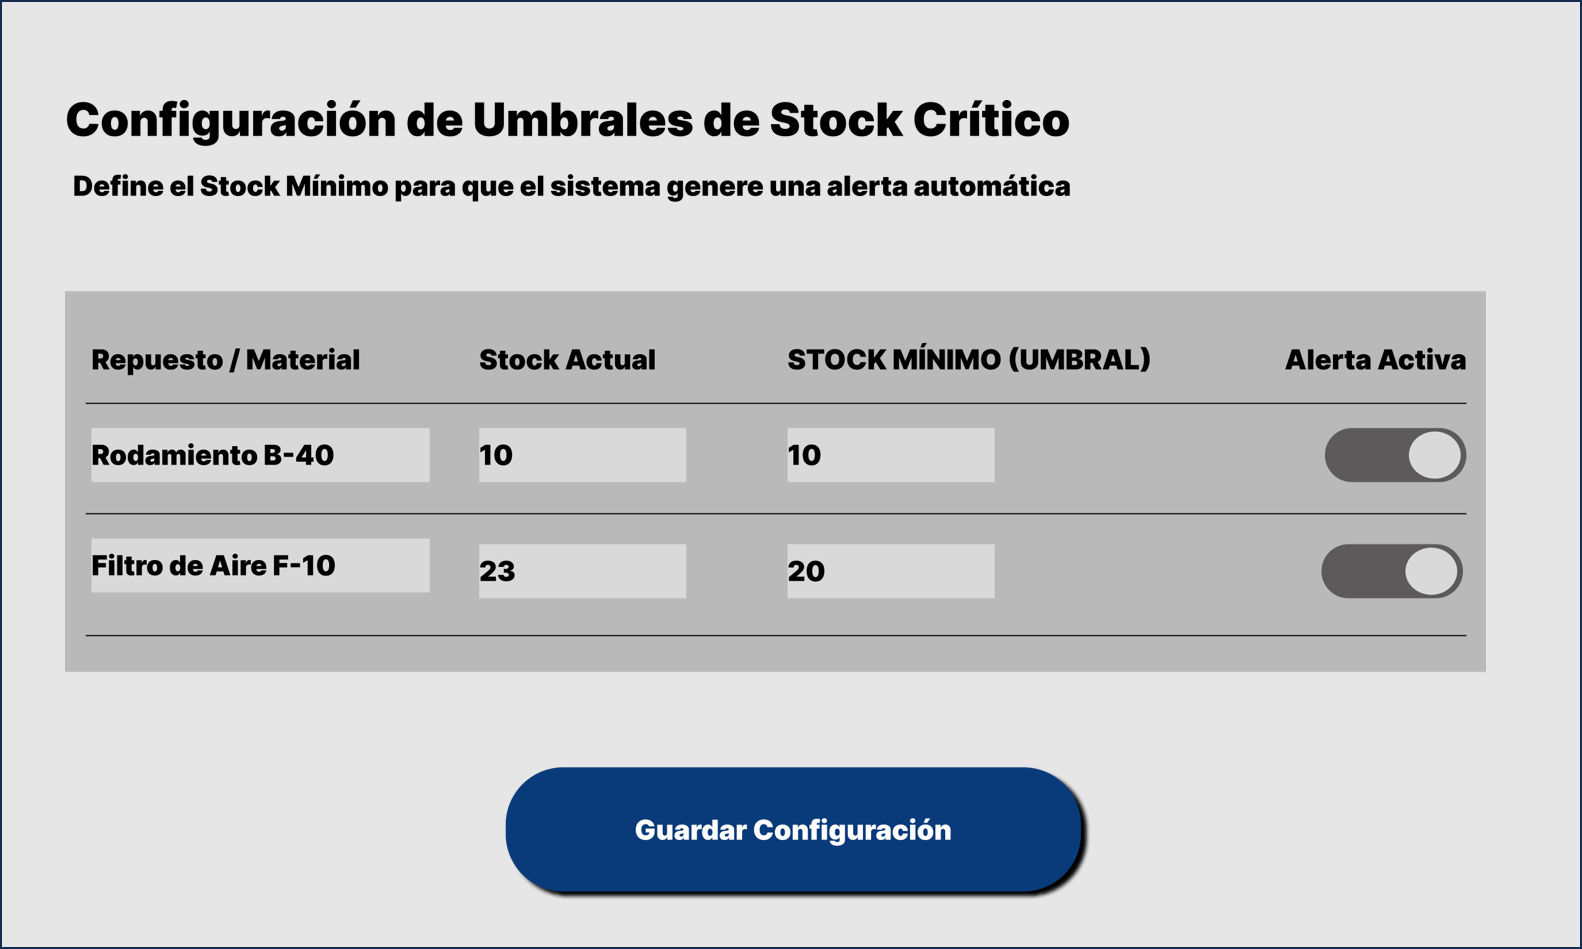
\includegraphics[width=0.9\textwidth]{assets/proto_twin.png}
    \caption{Prototipo P-INV-021}
\end{figure}

\begin{itemize}
    \item \textbf{Validación:} Se evidencia la \textbf{tabla de configuración} y el campo editable del \textbf{Stock Mínimo}, que permite al Jefe de Almacén definir el umbral de alerta.
\end{itemize}

\subsection{P-VIS-010: Visualización de Despiece 3D}

\begin{figure}[H]
    \centering
    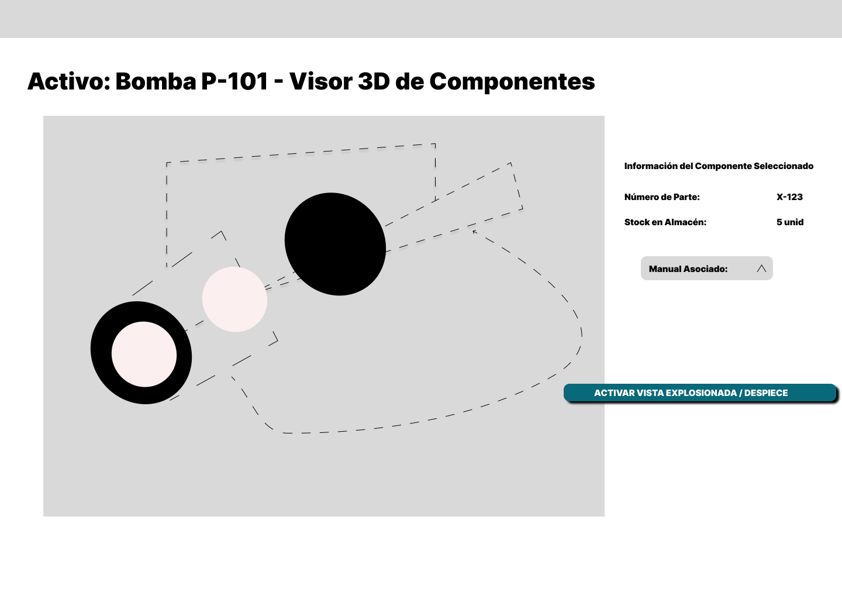
\includegraphics[width=0.9\textwidth]{assets/proto_wo.png}
    \caption{Prototipo P-VIS-010}
\end{figure}

\begin{itemize}
    \item \textbf{Validación:} La interfaz de escritorio muestra el área de visualización 3D y el botón para \textbf{activar la Vista Explosionada/Despiece}, requisito fundamental para el Técnico.
\end{itemize}

\section{Casos de Prueba (Validación Funcional)}

Las siguientes tablas detallan los Casos de Prueba diseñados para validar cada funcionalidad crítica de los prototipos.

\subsection{Caso de Prueba para MTTO-001 (Programación)}

\footnotesize
\begin{longtable}{|p{2cm}|p{2cm}|p{3cm}|p{2.5cm}|p{3cm}|p{3cm}|}
\hline
\textbf{ID Caso} & \textbf{Req. Asoc.} & \textbf{Objetivo} & \textbf{Pre-condiciones} & \textbf{Pasos} & \textbf{Resultado Esperado} \\ \hline
CP-MTTO-001 & MTTO-001 & Verificar la programación de mantenimiento con frecuencia trimestral. & El activo está registrado. & 1. Seleccionar activo. \newline 2. Seleccionar la frecuencia \textbf{``Trimestral''}. \newline 3. Ingresar Fecha de Inicio. \newline 4. Clic en ``Guardar Programación''. & El sistema crea la WO recurrente. Al navegar al calendario, se visualiza una nueva entrada de WO para el próximo trimestre. \\ \hline
\end{longtable}
\normalsize

\subsection{Caso de Prueba para ADM-017 (Dashboard)}

\footnotesize
\begin{longtable}{|p{2cm}|p{2cm}|p{3cm}|p{2.5cm}|p{3cm}|p{3cm}|}
\hline
\textbf{ID Caso} & \textbf{Req. Asoc.} & \textbf{Objetivo} & \textbf{Pre-condiciones} & \textbf{Pasos} & \textbf{Resultado Esperado} \\ \hline
CP-ADM-017 & ADM-017 & Verificar la visualización de los KPIs y el filtrado por rango de fechas. & Datos de mantenimiento de 6 meses cargados. & 1. Ingresar al Dashboard. \newline 2. Verificar que los KPIs (MTBF, MTTR) muestren valores. \newline 3. Aplicar el filtro ``Últimos 3 meses''. & Los widgets de KPI y los gráficos de tendencia \textbf{se actualizan dinámicamente} para mostrar únicamente los datos correspondientes al rango de `Últimos 3 meses'. \\ \hline
\end{longtable}
\normalsize

\subsection{Caso de Prueba para INV-021 (Alertas Stock)}

\footnotesize
\begin{longtable}{|p{2cm}|p{2cm}|p{3cm}|p{2.5cm}|p{3cm}|p{3cm}|}
\hline
\textbf{ID Caso} & \textbf{Req. Asoc.} & \textbf{Objetivo} & \textbf{Pre-condiciones} & \textbf{Pasos} & \textbf{Resultado Esperado} \\ \hline
CP-INV-021 & INV-021 & Validar que el sistema \textbf{genera una alerta} cuando el stock cae por debajo del umbral configurado. & Permisos de Jefe de Almacén. & 1. Establecer el umbral de `Rodamiento B-40' en 5. \newline 2. \textbf{Simular una salida de almacén de 1 unidad} (stock actual queda en 4). & El sistema debe generar una \textbf{notificación inmediata} (email o en-app) al Jefe de Almacén con el asunto `Alerta: Stock Crítico' \\ \hline
\end{longtable}
\normalsize

\subsection{Caso de Prueba para VIS-010 (Despiece 3D)}

\footnotesize
\begin{longtable}{|p{2cm}|p{2cm}|p{3cm}|p{2.5cm}|p{3cm}|p{3cm}|}
\hline
\textbf{ID Caso} & \textbf{Req. Asoc.} & \textbf{Objetivo} & \textbf{Pre-condiciones} & \textbf{Pasos} & \textbf{Resultado Esperado} \\ \hline
CP-VIS-010 & VIS-010 & Verificar la visualización 3D y la activación del modo Despiece. & El modelo 3D del activo está cargado. & 1. Abrir la vista 3D del activo. \newline 2. Clic en ``ACTIVAR VISTA EXPLOSIONADA''. \newline \textbf{3. Tocar un componente del modelo (ej. rodamiento).} & El modelo se separa visualmente. Al tocar el componente, \textbf{se muestra una tarjeta de información} con su número de parte y stock. \\ \hline
\end{longtable}
\normalsize

\section{Conclusiones}

La construcción de prototipos y el diseño de Casos de Prueba han permitido validar exitosamente los cuatro requerimientos críticos seleccionados. Este ejercicio confirma que las interfaces propuestas son lógicamente coherentes y que los flujos de trabajo son testables. Los artefactos generados constituyen una base sólida para la fase de diseño de alta fidelidad y el posterior desarrollo, mitigando el riesgo de construir funcionalidades que no se alinean con las necesidades del usuario.
